% Paper B, v2: rebuilt from the brief and the hypothesis work (September 2026).
\input{../../v3_rp/preamble}
\usepackage{longtable}
\usepackage{array}
\usepackage{placeins}
\graphicspath{{../../}}
\makeatletter\def\input@path{{./}{../../}{../../v3_rp/}}\makeatother
\title{\bfseries Where Being Unusual Pays and Being Early Costs\\
\large Evidence from 3.1 Million US Trademark Registrations}
\author{Eric Silver\thanks{Independent researcher, Pittsburgh, PA, USA.
ORCID 0000-0003-3351-1109. \texttt{eric.silver@aporal.com}.}}
\date{September 2026}

\begin{document}
\maketitle
\begin{abstract}
\noindent Strategy research disagrees about whether it pays to bring a new
kind of offering to market first, and a practitioner literature holds
that it pays to create uncontested market space. We compare the size of
the forces each side names on one outcome: whether a registered US
trademark's goods are still being sold at the sworn five-year proof of
continued use. Each of 3.1 million registrations from 2002--2018 is
scored on two positions of its goods-and-services language within its
industry: atypicality, how unusual the language is, and lead, whether
the industry later moved toward it. The most unusual filing in a class
and year passes the proof 5.4 points more often than the most typical;
the most leading passes 2.2 points less often than the most lagging;
both persist at the ten-year renewal. Twenty-four factors from the
filing record, curated vocabularies, emergent themes and the geography
of applicants change these values. The advantage of unusual language
roughly halves where the class's filing volume grows fast and where a
theme's filers are geographically concentrated; it doubles for owners
who patent. The cost of leading language disappears when counsel is
retained and reaches six points in platform businesses. Industries
differ stably: leading costs 8--11 points in tobacco and technology
services at both tests and is rewarded in construction, transport and
toys.

\medskip
\noindent\emph{Keywords:} first-mover advantage; blue ocean strategy;
trademarks; product survival; industry evolution; geographic clustering.
\end{abstract}

\section{Introduction}\label{sec:intro}

\emph{Pioneers keep the markets they open.} In surveys of consumer-goods
businesses, market pioneers held larger shares than early followers, and
early followers larger than late entrants \citep{RobinsonFornell1985}. A
pioneer can stay ahead in technology and learning, take scarce inputs
before others arrive, and hold customers who would pay to switch
\citep{LiebermanMontgomery1988}; when a new industry is later winnowed,
the early entrants are the likeliest to survive the shakeout
\citep{KlepperMiller1995, Klepper1997}.

\emph{Most pioneers fail, and followers take what they proved.} Where an
innovation is easy to imitate and the assets needed to sell it belong to
others, imitators capture its value \citep{Teece1986}. The histories of
fifty product categories showed that about half of the true first
entrants failed and that the firms remembered as pioneers had usually
entered later \citep{GolderTellis1993}; in consulting, rivals copy new
offerings routinely \citep{SemadeniAnderson2010}. Whether moving first
pays depends on the resources the entrant brings
\citep{LiebermanMontgomery1998} and on how fast technology and demand
change \citep{SuarezLanzolla2007}.

\emph{Creating a new category pays.} A practitioner literature holds that
firms which create uncontested market space, often by combining
attributes from different industries, grow faster and earn more than
those that compete in existing categories \citep{KimMauborgne2004}.

These claims are usually argued against one another, each from its own
cases. The trademark record makes it possible to measure the forces they
name together, on one outcome, for every entrant including those that
failed, and so to ask a different question: how large is each force, and
what changes it? A US trademark registration carries a dated description
of the goods or services the mark covers. Between the fifth and sixth
year after registration the owner must swear that the mark is still in
use in commerce, or the registration is cancelled; the five-year proof
is therefore a record of whether the product was still being sold. We
score each registration's description on two positions within its
industry \citep{SilverCorpus2026}: \emph{atypicality}, how unusual the
language is against the filings before and after it, and \emph{lead},
whether the industry's later filings moved toward it.

Four results organize the paper. First, the two positions pull in
opposite directions. The most unusual filing in its class and year
passes the proof 5.4 points more often than the most typical; the most
leading passes 2.2 points less often than the most lagging; both
effects hold at the ten-year renewal. Second, the advantage of unusual
language is real but fragile. It is about 6 points where a class's
filing volume is growing slowly and about 3 where it is growing fast,
and it falls from 6.2 to 2.8 points as the filers of the same theme
become more concentrated in place. Third, it can be protected: owners
who patent keep 7.6 points of it against 3.7 for owners who do not.
Fourth, the cost of being early is concentrated. It is near zero for
counsel-represented filings and 5.1 points for self-filed ones; it
reaches 6 points for platform businesses; and it is large and lasting in
a dozen classes, from tobacco to technology services, while it turns
into a reward in construction, transport and toys.

Section~\ref{sec:data} describes the registrations, the two positions
and the factors, and explains which factors come from curated
vocabularies and which from themes the data produced unaided.
Section~\ref{sec:headline} reports the two positions.
Section~\ref{sec:magnitudes} compares the factors on one scale.
Sections~\ref{sec:blue} and~\ref{sec:protect} report what erodes and
what protects the value of unusual language, and what changes the cost
of early language. Section~\ref{sec:geo} builds and applies a measure of
geographic clustering. Section~\ref{sec:industries} maps the results by
industry and follows them to renewal. Section~\ref{sec:discussion}
discusses what the magnitudes imply.

\section{Registrations, positions and factors}\label{sec:data}

\subsection{Registrations and outcomes}

The unit is the registration: 3,104,534 US trademark registrations issued
2002--2018, each counted once in its lowest Nice class (the international
classification's 45 classes of goods and services). The main outcome is
survival of the five-year proof: a registration passes unless it was
cancelled for want of the declaration between 4.0 and 8.5 years after
registration. 47.7\% of registrations pass. The second outcome is
renewal at year ten among registrations that passed the proof, observed
for the 871,819 registrations of 2002--2013 that reached a terminal
status; 59.9\% were renewed. For the capital-markets outcomes, the unit
is the owner's first registered filing, linked by name to private-offering
notices and to listings \citep{SilverCorpus2026}.

\subsection{Two positions of the language}

A topic model reduces every goods-and-services description to a mix of
fifty themes. For each filing, the mix is compared by Kullback--Leibler
divergence with the mix of its own class's filings in the five years
before its filing date and in the five years after. Atypicality is the
average of the two divergences: how far the filing's language sits from
its industry's, looking both ways. Lead is their difference: positive
when the filing is closer to what its class filed afterwards than to
what it had filed before, so that the industry moved toward it. Within a
class and year the two are nearly uncorrelated ($r = -0.10$). Both are
used here as percentiles within Nice class and registration year, so an
effect is the difference between the top and the bottom of that
distribution.

The theme model is fitted once on all classes together. Under such a
model a filing that carries a theme common in other classes but rare in
its own registers as atypical, and a model fitted within each class does
not register it; the survival advantage of atypicality is largely a
reading of such imported themes \citep{SilverCorpus2026}. That is the
content of atypicality in this paper: language that brings to a class
what other industries describe and this one rarely does. It is close to
what the blue-ocean literature calls reconstructing market boundaries by
looking across industries \citep{KimMauborgne2004}.

\subsection{Emergent themes and forced vocabularies}\label{sec:themes}

Two kinds of content measure enter the analysis, and they answer
different questions. \emph{Emergent} measures come from the fifty themes
the topic model found without guidance: atypicality and lead
themselves; each filing's primary theme, the theme its description
draws on most; whether that theme was imported from another class;
how volatile the theme's share of its class has been; how much of its
growth came from first-time filers; the turnover of the class's whole
theme mix; and the geographic groups of Section~\ref{sec:geo}, which
are the filers of one primary theme in one class. Emergent themes cover
every filing and impose no prior view of which products matter, but they
are broad; a theme covers many products.

\emph{Forced} measures are curated lists of terms matched in the
description (Appendix~\ref{app:vocab}): the vocabularies of
general-purpose technologies (internet, mobile apps, cloud, social
media, artificial intelligence, blockchain), of named inventions (3D
printing, drones, virtual reality, electric vehicles, gene therapy,
nanotechnology), of emergent consumer categories (e-cigarettes, energy
drinks, kombucha, cold brew, plant-based milk, hard seltzer, CBD), and
of kinds of business (site-based, contract or subscription, platform).
Forced vocabularies name products a reader recognizes and can be dated:
a vocabulary \emph{arrives} in a class in the first year at least five
of the class's filings use it, which is what the pioneer-and-follower
comparison of Section~\ref{sec:blue} requires. They are chosen with
hindsight, because these products became important, so they describe
the fate of entrants into markets that turned out to matter, not a
random draw of new products.

\subsection{Factors and estimation}

Table~\ref{tab:factors} lists the twenty-four factors, their source and
their frequency. Every model is a linear probability model of passing
the proof with class $\times$ registration-year fixed effects, so each
comparison is within an industry and year; the controls are log
description length, log owner filing count and foreign-basis flags; and
standard errors are clustered by owner, because an owner files many
marks and abandons them together. Each factor enters three times: as a
main effect, and interacted with atypicality and with lead, so that it
can change what either position is worth. Factors are centred, so the
atypicality and lead effects are those of a registration of average
composition. Significance stars use Holm-adjusted $p$-values within each
panel of each column.

\begin{small}
\begin{longtable}{>{\raggedright\arraybackslash}p{4.3cm}lr>{\raggedright\arraybackslash}p{6.6cm}}
\caption{The factors, where each comes from, and how common it is}\label{tab:factors}\\
\toprule Factor & Source & Share & Definition \\ \midrule \endfirsthead
\toprule Factor & Source & Share & Definition \\ \midrule \endhead
Represented by counsel & Record & 78\% & An attorney of record on the application. \\
Owner files patents & Record & 20\% & The owner, matched by name, holds US patents (PatentsView). \\
Owner's first-ever filing & Record & 33\% & The owner's first filing in the record. \\
Owner has 25+ earlier filings & Record & 20\% & The owner had filed 25 or more marks before this one. \\
Intent-to-use filing & Record & 41\% & Filed on an intent-to-use basis rather than on use in commerce. \\
Foreign owner (not China) & Record & 18\% & Owner domiciled outside the US, other than China. \\
Owner in China & Record & 3\% & Owner domiciled in China. \\
Site-based offering (stores, restaurants, clinics) & Forced & 9\% & Description names a physical site: store, restaurant, hotel, clinic, salon, gym and similar. \\
Contract or subscription offering & Forced & 5\% & Description names a subscription, membership, account, insurance, banking or leasing. \\
Platform or network offering & Forced & 2\% & Description names a platform, marketplace, social network, online community or peer-to-peer service. \\
General-purpose-technology vocabulary & Forced & 15\% & Internet, mobile-app, cloud, social-media, artificial-intelligence or blockchain vocabulary. \\
New-invention vocabulary & Forced & 0.4\% & 3D printing, drone, virtual-reality, electric-vehicle, gene-therapy or nanotechnology vocabulary. \\
Emergent consumer-category vocabulary & Forced & 0.4\% & E-cigarette, energy-drink, kombucha, cold-brew, plant-milk, hard-seltzer or CBD vocabulary. \\
Primary theme imported from another class & Emergent & 5\% & The filing's primary theme held under 1\% of its class in the five prior years and at least 5\% of another class. \\
Theme-share volatility (per SD) & Emergent & SD & Year-to-year variability of the primary theme's share of its class, over the filing year $\pm 5$. \\
Theme growth from first-time filers (per SD) & Emergent & SD & Share of the primary theme's filings in its class over the next five years made by first-time filers. \\
Class theme-mix turnover (per SD) & Emergent & SD & Change in the class's theme mix between the five years before and after the filing year. \\
Theme's geographic co-location (per SD) & Geography & SD & Co-location index of the class's US filers of the same primary theme within two years of the filing (Section 7). \\
Theme has a geographic hub & Geography & 28\% & That group of filers has at least one hub (Section 7). \\
Filer located in a hub & Geography & 5\% & The filer is located in such a hub. \\
Class filing-volume growth (per SD) & Record & SD & Growth in the class's filing volume, five years after against five years before. \\
Filing year (per SD, about 5 years) & Record & SD & Filing year. \\
Filed in a boom (1998-2000, 2005-07) & Record & 19\% & Filed in 1998--2000 or 2005--07. \\
Filed in a bust (2001-02, 2008-09) & Record & 18\% & Filed in 2001--02 or 2008--09. \\
\bottomrule
\multicolumn{4}{p{14.2cm}}{\footnotesize Record: a field of the filing or the owner's filing history. Forced: a curated list of terms matched in the description (Appendix~\ref{app:vocab}). Emergent: derived from the fifty themes the topic model found without guidance. Geography: from the applicant's ZIP code. Share: percentage of the 3.10 million registrations with the factor; SD marks continuous factors.} \\
\end{longtable}\end{small}


\section{Unusual language pays and early language costs, at every stage
after registration}\label{sec:headline}

\emph{The two positions move survival in opposite directions}
(Figure~\ref{fig:headline}). Survival at the proof rises from 45.4\% in
the most typical tenth of a class and year to 50.9\% in the most unusual,
and falls from 48.7\% in the most lagging tenth to 45.6\% in the most
leading. In the regression with class-by-year fixed effects and
controls (Table~\ref{tab:reg}, column 1), the most unusual filing passes
the proof 5.4 points more often than the most typical, and the most
leading 2.2 points less often than the most lagging. The two effects do
not depend on each other: the interaction is $-0.4$ points and not
distinguishable from zero.

\begin{figure}[htbp]
\centering
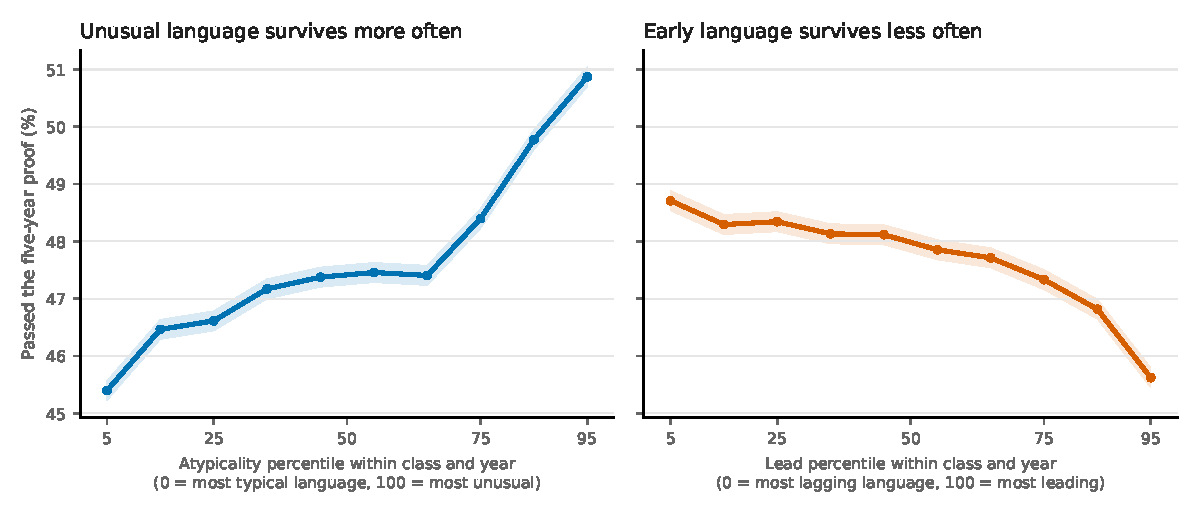
\includegraphics[width=\textwidth]{figures/fig_b_headline.pdf}
\caption{Share of registrations passing the five-year proof by tenth of
atypicality (left) and of lead (right), both measured within Nice class
and registration year. Survival is adjusted for class $\times$
registration-year fixed effects; bands are 95\% intervals.
3.10 million registrations, 2002--2018.}
\label{fig:headline}
\end{figure}

\emph{Both effects persist at the ten-year renewal.} Among registrations
that passed the proof, the most unusual is renewed 4.3 points more often
than the most typical and the most leading 0.9 points less often than
the most lagging. The advantage of unusual language keeps most of its
size; the cost of early language keeps less than half.

\emph{Unusual language is harder to register and early language easier.}
Among first-time filers, one standard deviation of atypicality lowers the
chance of registration by 1.0 point, and one standard deviation of lead
raises it by 0.5 (Table~\ref{tab:stages}). Examination screens against
unusual descriptions and passes descriptions that match where the class
is going; the market then reverses both.

\begin{table}[htbp]\centering\small
\caption{The two positions at each stage (first-time filers)}\label{tab:stages}
\begin{tabular}{lrr}
\toprule
Stage (points per standard deviation) & Atypicality & Lead \\
\midrule
Registered, of all filed & $-0.98$ & $+0.47$ \\
Passed the five-year proof, of registered & $+1.31$ & $-0.97$ \\
Renewed at year ten, of those that passed & $+1.38$ & $-0.43$ \\
Filed a private-offering notice, of registered & $-0.17$ & $-0.32$ \\
Listed after the offering, of those that filed one & $+0.87$ & $-0.53$ \\
\bottomrule
\end{tabular}
\par\footnotesize One row per owner (the owner's first scored filing);
class $\times$ first-filing-year fixed effects; log description length
held. All coefficients differ from zero at $p<0.001$.
\end{table}

\emph{Capital markets agree with the proof.} Owners whose first
registration led are less likely to file a private-offering notice
($-0.32$ points per SD, on a base of 2.5\%) and, among those that did,
less likely to list ($-0.53$ on a base of 3.5\%). Unusual first
registrations are slightly less likely to raise private money and more
likely to list once they have.

\section{The magnitude of each factor}\label{sec:magnitudes}

\emph{Counsel is the largest single factor, larger than either position.}
Figure~\ref{fig:magnitudes} places every factor on one scale, each
estimated alone with atypicality and lead. Registrations with an
attorney of record pass the proof 18.7 points more often than those
without. The next largest are the owner's filing history (owners with
25 or more earlier marks pass 12.5 points less often, because large
portfolios let more marks lapse; first-time filers 5.1 less often), the
filing basis (intent-to-use filings 6.0 less often), and what the filing
describes: emergent consumer categories pass 13.9 points less often,
new-invention vocabulary 7.8, platform businesses 8.9, and
general-purpose-technology vocabulary 5.4. Site-based businesses pass
2.0 points more often. Owners who patent pass 3.0 points less often; as
with large portfolios, patenting marks a larger firm with more marks to
let go.

\begin{figure}[htbp]
\centering
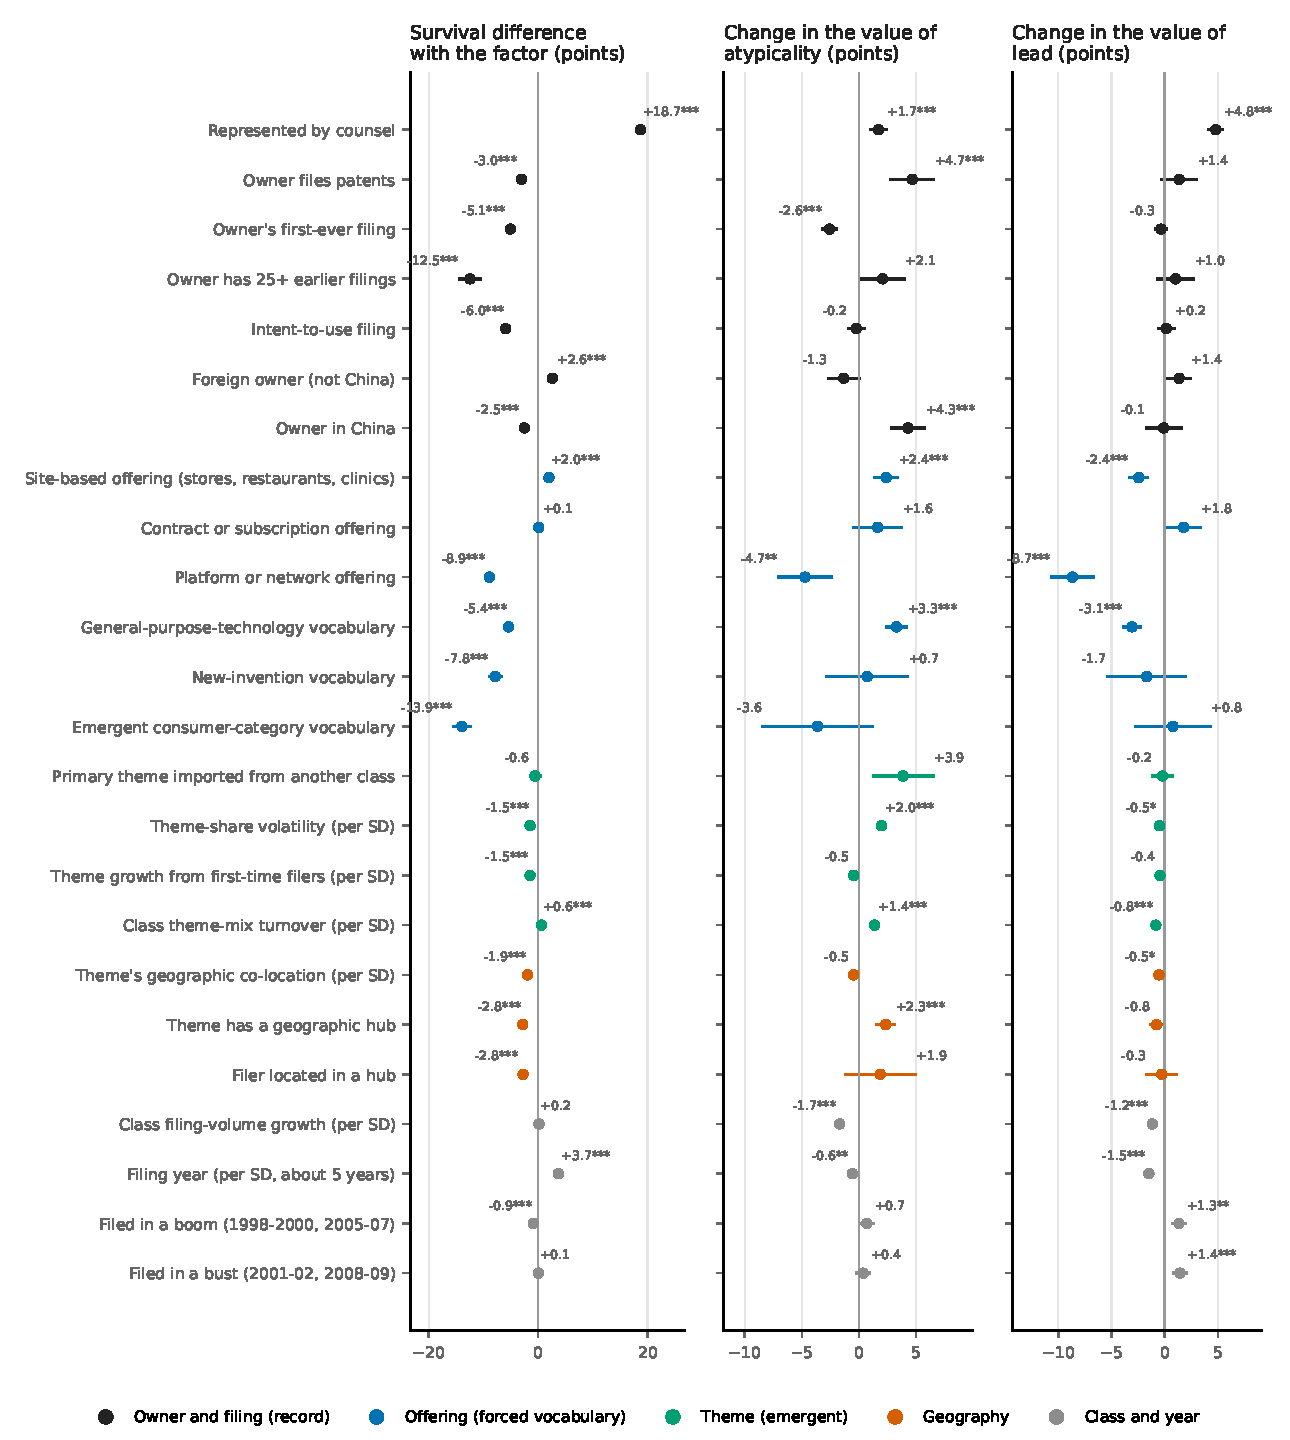
\includegraphics[width=\textwidth]{figures/fig_b_magnitudes.pdf}
\caption{Each factor estimated alone, with atypicality, lead and their
interaction and the controls. Left: difference in the share passing the
five-year proof between registrations with and without the factor
(continuous factors: per standard deviation). Centre and right: how much
the factor adds to or subtracts from the atypicality effect and the lead
effect (both measured as top minus bottom of the class-and-year
distribution). Lines are 95\% intervals; stars are Holm-adjusted within
each panel ($^{*}<0.05$, $^{**}<0.01$, $^{***}<0.001$). Colour marks
where the factor comes from (Table~\ref{tab:factors}).}
\label{fig:magnitudes}
\end{figure}

\emph{Half of the raw cost of leading is composition.} Adding the
factors lowers the cost of leading from 2.2 points to 1.2
(Table~\ref{tab:reg}, columns 1 and 3): leading filings are more often
self-filed, more often platforms and more often in general-purpose
technology vocabulary, and each of these survives less. The advantage of
atypicality changes less, from 5.4 to 4.5 points. Seventeen of the
twenty-four factors have at least one term that survives the adjustment
for multiple testing (column 2); dropping the other seven moves the
atypicality and lead effects by about a tenth of a point.

\emph{Where a factor changes the value of a position, it is more often
the value of atypicality than the cost of lead.} Eight factors change
the atypicality effect after adjustment; four change the lead effect
(Table~\ref{tab:reg}, panels B and C). Sections~\ref{sec:blue}
and~\ref{sec:protect} take them in turn.

\clearpage
\begin{small}
\begin{longtable}{>{\raggedright\arraybackslash}p{5.9cm}rrr}
\caption{Passing the five-year proof: atypicality, lead and the factors that change what each is worth}\label{tab:reg}\\
\toprule & (1) Atypicality & (2) With & (3) With all \\ & and lead only & significant factors & factors \\ \midrule
\endfirsthead
\toprule & (1) & (2) & (3) \\ \midrule \endhead
\multicolumn{4}{l}{\textbf{A. Survival difference (percentage points)}} \\
Atypicality (most unusual $-$ most typical) & +5.43$^{***}$ (0.24) & +4.61$^{***}$ (0.21) & +4.48$^{***}$ (0.22) \\
Lead (most leading $-$ most lagging) & $-$2.21$^{***}$ (0.21) & $-$1.15$^{***}$ (0.23) & $-$1.18$^{***}$ (0.24) \\
\quad Represented by counsel & & +18.70$^{***}$ (0.16) & +18.71$^{***}$ (0.16) \\
\quad Owner files patents & & $-$1.85$^{***}$ (0.38) & $-$1.86$^{***}$ (0.38) \\
\quad Owner's first-ever filing & & $-$1.09 (0.60) & $-$1.09 (0.60) \\
\quad Owner has 25+ earlier filings & & $-$10.29$^{***}$ (1.12) & $-$10.29$^{***}$ (1.12) \\
\quad Intent-to-use filing & & $-$6.88$^{***}$ (0.13) & $-$6.79$^{***}$ (0.14) \\
\quad Foreign owner (not China) & &  & +0.99 (0.61) \\
\quad Owner in China & & +0.74 (0.41) & +1.62 (0.61) \\
\quad Site-based offering (stores, restaurants, clinics) & & +2.26$^{***}$ (0.19) & +2.24$^{***}$ (0.19) \\
\quad Contract or subscription offering & &  & +0.00 (0.34) \\
\quad Platform or network offering & & $-$5.59$^{***}$ (0.43) & $-$5.60$^{***}$ (0.43) \\
\quad General-purpose-technology vocabulary & & $-$4.69$^{***}$ (0.16) & $-$4.66$^{***}$ (0.16) \\
\quad New-invention vocabulary & & $-$6.39$^{***}$ (0.62) & $-$6.42$^{***}$ (0.62) \\
\quad Emergent consumer-category vocabulary & & $-$12.16$^{***}$ (0.90) & $-$12.17$^{***}$ (0.90) \\
\quad Primary theme imported from another class & &  & +0.98 (0.57) \\
\quad Theme-share volatility (per SD) & & $-$0.83$^{***}$ (0.10) & $-$0.91$^{***}$ (0.10) \\
\quad Theme growth from first-time filers (per SD) & & $-$1.14$^{***}$ (0.13) & $-$1.13$^{***}$ (0.13) \\
\quad Class theme-mix turnover (per SD) & & +0.68$^{***}$ (0.13) & +0.60$^{***}$ (0.13) \\
\quad Theme's geographic co-location (per SD) & & $-$1.29$^{***}$ (0.10) & $-$1.30$^{***}$ (0.10) \\
\quad Theme has a geographic hub & & $-$0.46 (0.20) & $-$0.46 (0.24) \\
\quad Filer located in a hub & &  & +0.05 (0.52) \\
\quad Class filing-volume growth (per SD) & & +0.23 (0.11) & +0.27 (0.12) \\
\quad Filing year (per SD, about 5 years) & &  & +0.48 (0.32) \\
\quad Filed in a boom (1998-2000, 2005-07) & &  & $-$0.37 (0.19) \\
\quad Filed in a bust (2001-02, 2008-09) & &  & $-$0.09 (0.17) \\
\addlinespace\multicolumn{4}{l}{\textbf{B. Change in the value of atypicality (points)}} \\
Lead & $-$0.37 (0.54) & $-$1.10 (0.59) & $-$0.75 (0.59) \\
\quad Represented by counsel & & +0.20 (0.35) & +0.25 (0.36) \\
\quad Owner files patents & & +3.79$^{***}$ (0.90) & +3.91$^{***}$ (0.89) \\
\quad Owner's first-ever filing & & $-$1.74$^{***}$ (0.27) & $-$1.68$^{***}$ (0.28) \\
\quad Owner has 25+ earlier filings & & $-$0.65 (0.79) & $-$0.76 (0.80) \\
\quad Intent-to-use filing & & $-$0.22 (0.34) & $-$0.30 (0.35) \\
\quad Foreign owner (not China) & &  & $-$1.53 (0.78) \\
\quad Owner in China & & +6.01$^{***}$ (0.78) & +5.88$^{***}$ (0.79) \\
\quad Site-based offering (stores, restaurants, clinics) & & +2.67$^{***}$ (0.55) & +2.74$^{***}$ (0.56) \\
\quad Contract or subscription offering & &  & $-$0.80 (1.16) \\
\quad Platform or network offering & & $-$4.14$^{**}$ (1.24) & $-$3.76 (1.29) \\
\quad General-purpose-technology vocabulary & & +1.99$^{**}$ (0.54) & +2.13$^{***}$ (0.48) \\
\quad New-invention vocabulary & & $-$3.51 (1.77) & $-$3.08 (1.78) \\
\quad Emergent consumer-category vocabulary & & $-$1.46 (2.48) & $-$1.64 (2.48) \\
\quad Primary theme imported from another class & &  & +0.85 (1.41) \\
\quad Theme-share volatility (per SD) & & +0.81$^{***}$ (0.20) & +0.37 (0.22) \\
\quad Theme growth from first-time filers (per SD) & & +0.27 (0.22) & +0.15 (0.25) \\
\quad Class theme-mix turnover (per SD) & & +0.21 (0.19) & +0.32 (0.18) \\
\quad Theme's geographic co-location (per SD) & & $-$1.77$^{***}$ (0.22) & $-$1.72$^{***}$ (0.23) \\
\quad Theme has a geographic hub & & +2.86$^{***}$ (0.53) & +2.12$^{***}$ (0.52) \\
\quad Filer located in a hub & &  & +1.62 (1.65) \\
\quad Class filing-volume growth (per SD) & & $-$1.54$^{***}$ (0.19) & $-$1.53$^{***}$ (0.19) \\
\quad Filing year (per SD, about 5 years) & &  & $-$0.30 (0.21) \\
\quad Filed in a boom (1998-2000, 2005-07) & &  & +0.03 (0.41) \\
\quad Filed in a bust (2001-02, 2008-09) & &  & $-$0.63 (0.43) \\
\addlinespace\multicolumn{4}{l}{\textbf{C. Change in the value of lead (points)}} \\
\quad Represented by counsel & & +5.17$^{***}$ (0.36) & +5.05$^{***}$ (0.37) \\
\quad Owner files patents & & +0.33 (0.73) & +0.29 (0.73) \\
\quad Owner's first-ever filing & & +0.73 (0.26) & +0.72 (0.27) \\
\quad Owner has 25+ earlier filings & & $-$0.15 (0.69) & $-$0.07 (0.69) \\
\quad Intent-to-use filing & & $-$0.82 (0.35) & $-$0.97 (0.36) \\
\quad Foreign owner (not China) & &  & +0.62 (0.63) \\
\quad Owner in China & & +0.68 (0.84) & +1.37 (0.86) \\
\quad Site-based offering (stores, restaurants, clinics) & & $-$1.26 (0.47) & $-$1.33 (0.47) \\
\quad Contract or subscription offering & &  & +1.92 (0.82) \\
\quad Platform or network offering & & $-$4.87$^{***}$ (1.08) & $-$4.88$^{***}$ (1.09) \\
\quad General-purpose-technology vocabulary & & $-$2.11$^{***}$ (0.45) & $-$2.12$^{***}$ (0.44) \\
\quad New-invention vocabulary & & $-$1.27 (1.90) & $-$1.00 (1.92) \\
\quad Emergent consumer-category vocabulary & & $-$0.93 (1.85) & $-$0.55 (1.85) \\
\quad Primary theme imported from another class & &  & $-$0.56 (0.58) \\
\quad Theme-share volatility (per SD) & & +0.42 (0.20) & +0.37 (0.21) \\
\quad Theme growth from first-time filers (per SD) & & +0.01 (0.23) & +0.14 (0.23) \\
\quad Class theme-mix turnover (per SD) & & $-$0.65$^{***}$ (0.16) & $-$0.77$^{***}$ (0.18) \\
\quad Theme's geographic co-location (per SD) & & $-$0.24 (0.18) & $-$0.27 (0.19) \\
\quad Theme has a geographic hub & & $-$0.28 (0.38) & +0.06 (0.46) \\
\quad Filer located in a hub & &  & +0.03 (0.77) \\
\quad Class filing-volume growth (per SD) & & $-$0.60$^{*}$ (0.19) & $-$0.34 (0.21) \\
\quad Filing year (per SD, about 5 years) & &  & $-$0.55 (0.25) \\
\quad Filed in a boom (1998-2000, 2005-07) & &  & +0.64 (0.47) \\
\quad Filed in a bust (2001-02, 2008-09) & &  & +0.16 (0.42) \\
\addlinespace\midrule
Registrations & 3,104,534 & 3,104,534 & 3,104,534 \\
Factors & 0 & 17 & 24 \\
\bottomrule
\multicolumn{4}{p{14.2cm}}{\footnotesize Linear probability models of passing the five-year proof of continued use, registrations 2002--2018. Atypicality and lead are percentiles within Nice class and registration year, centred, so a coefficient in panel A is the difference between the top and the bottom of the class-and-year distribution. Factors are centred (binary factors 0/1, continuous factors in SD units), so the atypicality and lead rows are the effects for a registration of average composition. Panel B reports how much a factor adds to or subtracts from the atypicality effect; panel C, from the lead effect. Column 2 keeps the factors with at least one term significant in column 3. All models: class $\times$ registration-year fixed effects; log description length, log owner filing count and foreign-basis flags; standard errors clustered by owner in parentheses. Stars: Holm-adjusted $p$ within each panel of each column; $^{*}<0.05$, $^{**}<0.01$, $^{***}<0.001$.} \\
\end{longtable}
\end{small}


\section{The advantage of unusual language, and what erodes it}\label{sec:blue}

\emph{A blue-ocean effect exists, and it lasts.} With every factor held,
the most unusual filing in its class and year passes the proof 4.5
points more often than the most typical, and among those that pass it is
renewed 4.3 points more often. Because atypicality under a single theme
model registers themes imported from other classes
(Section~\ref{sec:data}), the effect belongs to filings that describe, in
their class, what other industries describe. Flagging imported primary
themes directly adds nothing once atypicality is held ($+1.0$ points,
not significant): the advantage runs through how unusual the whole
description is, not through a single borrowed theme.

\emph{Growth in the class's filing volume erodes it.} Each standard
deviation of five-year growth in the class's filings reduces the
atypicality advantage by 1.5 points: it is worth 6.0 points one SD below
the mean and 3.0 one SD above. Figure~\ref{fig:blue}b shows where the
loss falls. In the fastest-growing third of class-years, survival is
nearly flat from the 10th to the 80th percentile of atypicality, about
one point above the most typical tenth, and rises only in the most
unusual fifth. In the slowest-growing third it rises across the whole
range.

\begin{figure}[htbp]
\centering
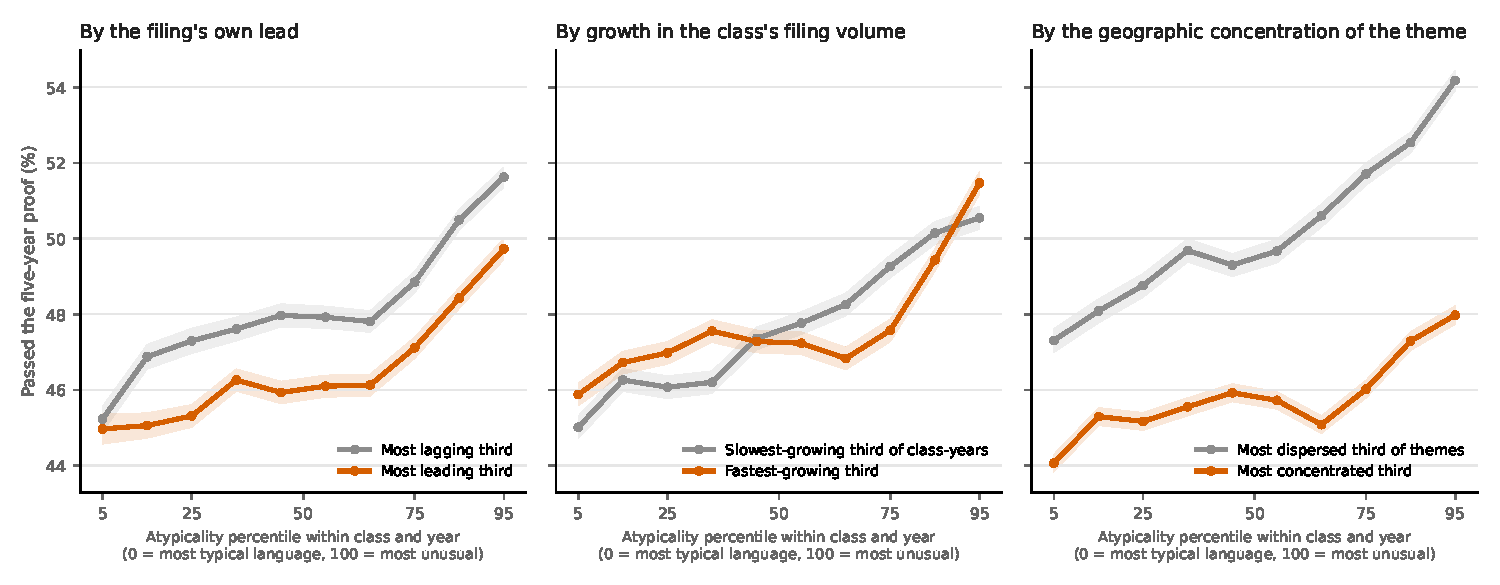
\includegraphics[width=\textwidth]{figures/fig_b_blueocean.pdf}
\caption{Share passing the five-year proof by tenth of atypicality, for
(a) the most lagging and most leading third of filings in their class
and year; (b) class-years in the slowest- and fastest-growing third of
filing volume (five years after against five years before); (c) themes
in the most dispersed and most concentrated third of geographic
co-location (Section~\ref{sec:geo}). Survival adjusted for class
$\times$ registration-year fixed effects; bands are 95\% intervals.}
\label{fig:blue}
\end{figure}

\emph{Geographic concentration erodes it more.} Each standard deviation
of a theme's co-location reduces the atypicality advantage by 1.7
points: from 6.2 points one SD below the mean to 2.8 one SD above. In
the raw comparison (Figure~\ref{fig:blue}c), unusual filings in the most
dispersed third of themes pass the proof 6.9 points more often than
typical ones; in the most concentrated third, 3.9. Section~\ref{sec:geo}
returns to this.

\emph{A filing's own lead does not change the advantage detectably.} The
most lagging third of filings gains 6.4 points from the most typical to
the most unusual tenth and the most leading third 4.7
(Figure~\ref{fig:blue}a), but the interaction in the regression is
$-0.8$ points and not distinguishable from zero, at the proof or at
renewal ($-1.4$, s.e.\ 0.9). What erodes the advantage is growth in the
class and concentration of the theme, not the filing's own position
ahead of its class.

\emph{First-time filers keep less of it.} For an owner's first filing the
atypicality advantage is 3.4 points; for later filings, 5.0.

\emph{Pioneers of a named product fail, and so do its early followers.}
The forced vocabularies can be dated. Filings using a vocabulary in its
arrival year or the year after pass the proof 12.8 points less often
than the other filings of their class and year; filings two to five
years after arrival, 11.8 points less often; later filings, 6.0 points
less often. The first two do not differ ($t = 0.5$). Pioneers fail, as
\citet{GolderTellis1993} found in fifty product histories; the early
followers here fail at the same rate.

\emph{Leading costs most where markets grow and technology turns over
together.} Dividing class-years at the median of theme-mix turnover and
of filing-volume growth, and holding a filing-year trend, leading costs
4.7 points where both change fast, 2.7 where only volume grows, 1.0 in
calm class-years and 0.8 where only the theme mix turns over. The
pace-of-change account predicts the most durable first-mover advantage
where the market grows and technology is stable
\citep{SuarezLanzolla2007}; the record puts a larger cost there than in
calm class-years.

\section{What protects the advantage, and what changes the cost of
leading}\label{sec:protect}

\emph{Patents double the advantage of unusual language.} For owners who
patent, the most unusual filing passes the proof 7.6 points more often
than the most typical; for owners who do not, 3.7 (Table~\ref{tab:reg},
panel B, $+3.9$ points; Figure~\ref{fig:protect}a). Patents do not change
the cost of leading ($+0.3$, not significant). Owners who can protect the
technology behind an unusual offering keep more of what it earns; the
protection does not extend to being early.

\begin{figure}[htbp]
\centering
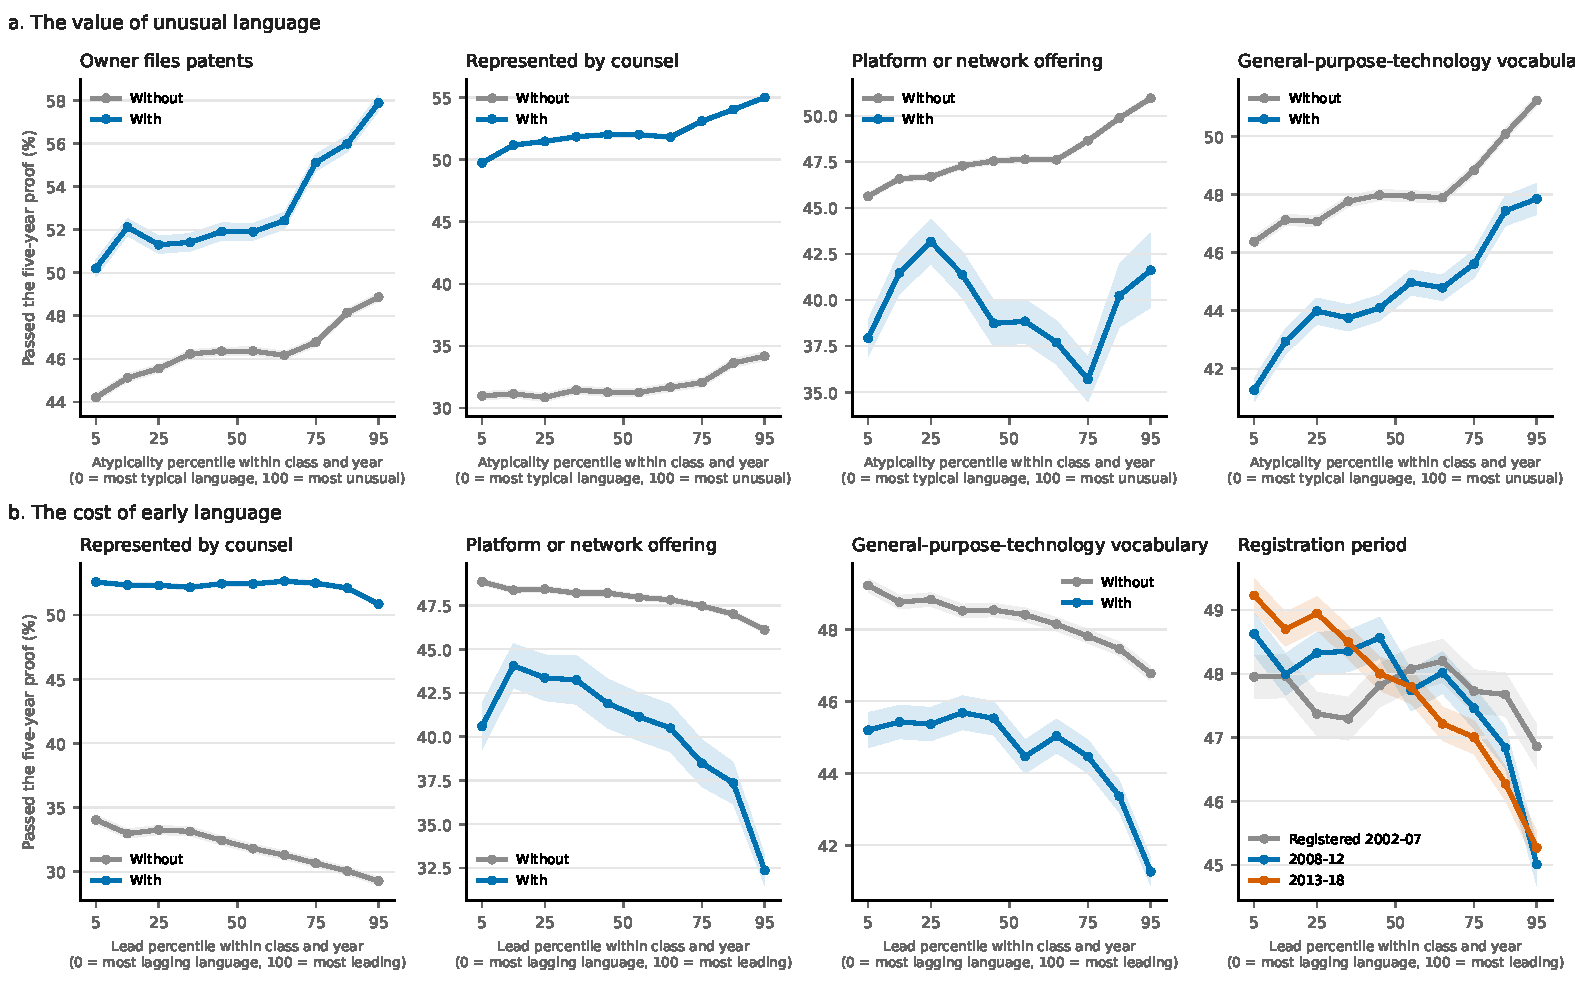
\includegraphics[width=\textwidth]{figures/fig_b_protect.pdf}
\caption{Share passing the five-year proof by tenth of atypicality (a)
and of lead (b), for registrations with and without each factor, and
(bottom right) by registration period. Survival adjusted for class
$\times$ registration-year fixed effects; bands are 95\% intervals.}
\label{fig:protect}
\end{figure}

\emph{Site-based businesses, general-purpose technologies and owners in
China also keep more of it.} The atypicality advantage is 7.0 points for
site-based businesses (4.2 for others), 6.3 for filings in
general-purpose-technology vocabulary (4.2), 6.0 for themes with a
geographic hub (3.9), and 10.2 for owners in China (4.3). For owners in
China the typical filing fares badly and the unusual one does not.

\emph{Platform businesses do not keep it.} For platform and network
offerings the atypicality advantage is 0.8 points, against 4.6 for other
filings; the difference ($-3.8$) does not survive the adjustment for
multiple testing, but it is the largest negative change in panel B.

\emph{Counsel removes the cost of leading.} Among counsel-represented
registrations the most leading filing passes the proof as often as the
most lagging ($-0.1$ points); among self-filed registrations, 5.1 points
less often (Figure~\ref{fig:protect}b). Counsel does not change the value
of unusual language ($+0.3$). At renewal, counsel still halves the cost of
leading ($+2.2$ points).

\emph{Platforms and general-purpose technologies pay more for leading.}
Leading costs platform businesses 6.0 points (1.1 for other filings) and
filings in general-purpose-technology vocabulary 3.0 (0.9). The platform
penalty persists at renewal ($-8.5$ against other filings); the extra
cost for general-purpose technology is paid at the proof and not at
renewal ($-0.6$, not significant).

\emph{The cost of leading has grown over time.} For registrations of
2002--07 the most leading filing passed the proof as often as the most
lagging ($-0.1$ points); for 2008--12 and 2013--18, 2.2 and 2.0 points less
often (Figure~\ref{fig:protect}b, right). Once a filing-year trend is
held, booms (1998--2000, 2005--07) and busts (2001--02, 2008--09) do not
differ from other years.

\section{Geographic clustering}\label{sec:geo}

\emph{A measure of clustering needs to allow several hubs and to net out
where firms are anyway.} Distance to the nearest neighbour or to a
single centre cannot recognize an industry split between the Bay Area
and New York, and every industry's filers concentrate where people and
firms are. We place each US applicant at the Census centroid of the ZIP
code on its application (re-parsed from the annual case-file archives;
99.8\% of US owners placed, 92\% at their own ZIP code) and measure a
group of $N$ filers by the average, over all pairs, of a distance kernel:
\[
C = \frac{1}{N(N-1)}\sum_{i \neq j} k(d_{ij}), \qquad
k(d) = \max\!\left(0,\; 1 - \frac{d}{200\text{ miles}}\right).
\]
Two filers in the same place score 1, two 100 miles apart 0.5, two more
than 200 miles apart 0; $C$ is the chance that two filers drawn at random
are neighbours, weighted by how near. Any number of hubs contributes: a
group split evenly between two distant cities scores half of what it
would in one. The same index for all filers in the same classes and
years gives the baseline $B$, and co-location is
$L = (C - B)/(1 - B)$: zero for a group placed like its classes, one when
every filer is in one place. This is the distance-based comparison with
a counterfactual of \citet{DurantonOverman2005}, summarized at one
bandwidth. A \emph{hub} is a place near which (kernel-weighted) at least
10\% of the group's filers sit, at least 1.2 times the share of all
filers there; hubs are taken in order of their share, each excluding
places within 200 miles of the last.

\emph{The measure recognizes industries with known geography}
(Figure~\ref{fig:geo}, Table~\ref{tab:geo}). Semiconductor filers of
1995--2005 have co-location 0.20, with 48\% of them near Santa Clara
against 12\% of all filers in their class. Social-networking filers of
2004--12 have three hubs, New York, San Francisco and Los Angeles.
Biotechnology filers cluster near Philadelphia, the Bay Area and New
Haven; casino filers near Las Vegas; country-music filers near
Nashville. Broad vocabularies used across the economy, such as internet
language in 1998--2001, show almost no co-location ($L = 0.01$).

\begin{figure}[htbp]
\centering
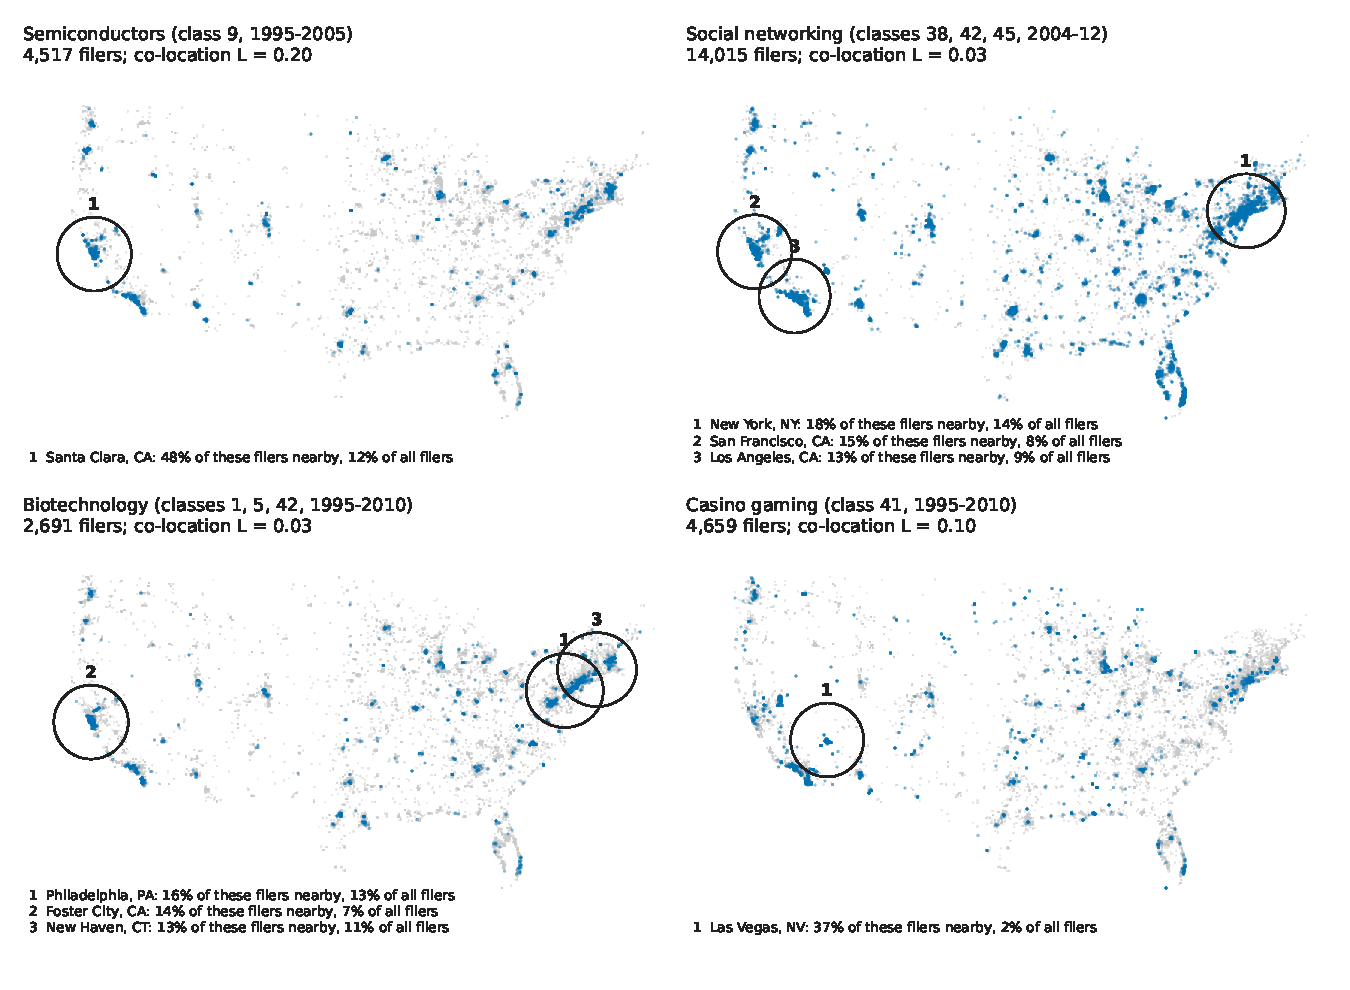
\includegraphics[width=\textwidth]{figures/fig_geo_map.pdf}
\caption{US filers whose descriptions use each vocabulary (blue), against
a sample of all filers in the same classes and years (grey). Circles are
the detected hubs, 200 miles in radius; the key gives the share of the
group and of all filers near each.}
\label{fig:geo}
\end{figure}

\begin{table}[htbp]\centering\small
\caption{The co-location measure on groups with known geography}\label{tab:geo}
\begin{tabular}{>{\raggedright\arraybackslash}p{4.8cm}rrr>{\raggedright\arraybackslash}p{5.4cm}}
\toprule Filers using the vocabulary of & Filers & $L$ & & Hubs: share of the group nearby / share of all filers \\ \midrule
internet vocabulary, classes 9/35/38/42, 1998-2001 & 60,903 & 0.014 & & San Francisco, CA 13\% / 10\% \\
semiconductors, class 9, 1995-2005 & 4,517 & 0.203 & & Santa Clara, CA 48\% / 12\% \\
wine, class 33, 2000-2010 & 18,799 & 0.056 & & Napa, CA 35\% / 26\% \\
country music, class 41, 1995-2010 & 163 & 0.041 & & Nashville, TN 28\% / 1\% \\
casino gaming, class 41, 1995-2010 & 4,662 & 0.095 & & Las Vegas, NV 37\% / 2\% \\
biotechnology, classes 1/5/42, 1995-2010 & 2,695 & 0.031 & & Philadelphia, PA 16\% / 13\%; Foster City, CA 14\% / 7\%; New Haven, CT 13\% / 11\% \\
social networking, classes 38/42/45, 2004-2012 & 14,041 & 0.033 & & New York, NY 18\% / 14\%; San Francisco, CA 15\% / 8\%; Los Angeles, CA 13\% / 9\% \\
online advertising, classes 35/42, 2005-2015 & 12,028 & 0.027 & & New York, NY 17\% / 14\%; San Francisco, CA 14\% / 7\%; Los Angeles, CA 12\% / 9\% \\
software as a service, class 42, 2008-2016 & 20,783 & 0.008 & & San Francisco, CA 15\% / 10\% \\
hip hop, classes 9/25/41, 1995-2010 & 507 & 0.058 & & New York, NY 29\% / 16\% \\
\bottomrule\end{tabular}
\par\footnotesize $L$: co-location of the group net of all filers in the same classes and years (0 = placed like the classes, 1 = all in one place). Nearby: kernel-weighted within 200 miles.
\end{table}


\emph{Clustering lowers survival and erodes the advantage of unusual
language; it does not change the cost of leading.} For the regressions,
each registration is assigned the co-location of its group: the class's
US filers of the same primary theme within two years of its filing. Each
standard deviation of co-location lowers survival by 1.3 points and the
atypicality advantage by 1.7 points; it changes the lead effect by
$-0.3$, not distinguishable from zero. A group with an identifiable hub
keeps more of the atypicality advantage ($+2.1$ points), and a filer
located in a hub fares no differently from one outside it, in survival
($+0.1$) or in either effect. Concentration in place reduces what an
unusual description is worth; being in the hub itself neither helps nor
hurts.

\section{Industries: where the cost of leading falls and whether it
lasts}\label{sec:industries}

\emph{Industries differ in a stable way.} Estimated class by class, the
lead effect at the proof and the lead effect at renewal correlate at
0.67 across classes, and the atypicality effects at 0.74
(Figure~\ref{fig:industries}). In twelve classes leading costs at least
2 points at both tests: most in tobacco and vaping (11.3 points at the
proof, 7.9 at renewal) and technology and science services (9.6 and
7.9), then medical devices, meat and dairy, lighting and heating, hand
tools and fabrics. In five it costs only at the proof: electronics and
software, advertising and business services, hotels and restaurants,
chemicals and clothing. In four it costs only at renewal: education and
entertainment, housewares, jewelry and fuels. Leading is rewarded at
both tests in construction and repair (4.0 and 4.5), transport and
storage, toys and sporting goods, firearms and treatment of materials,
and at the proof only in beer and soft drinks (9.6), paints and legal
services. Appendix~\ref{app:classes} lists every class.

\begin{figure}[htbp]
\centering
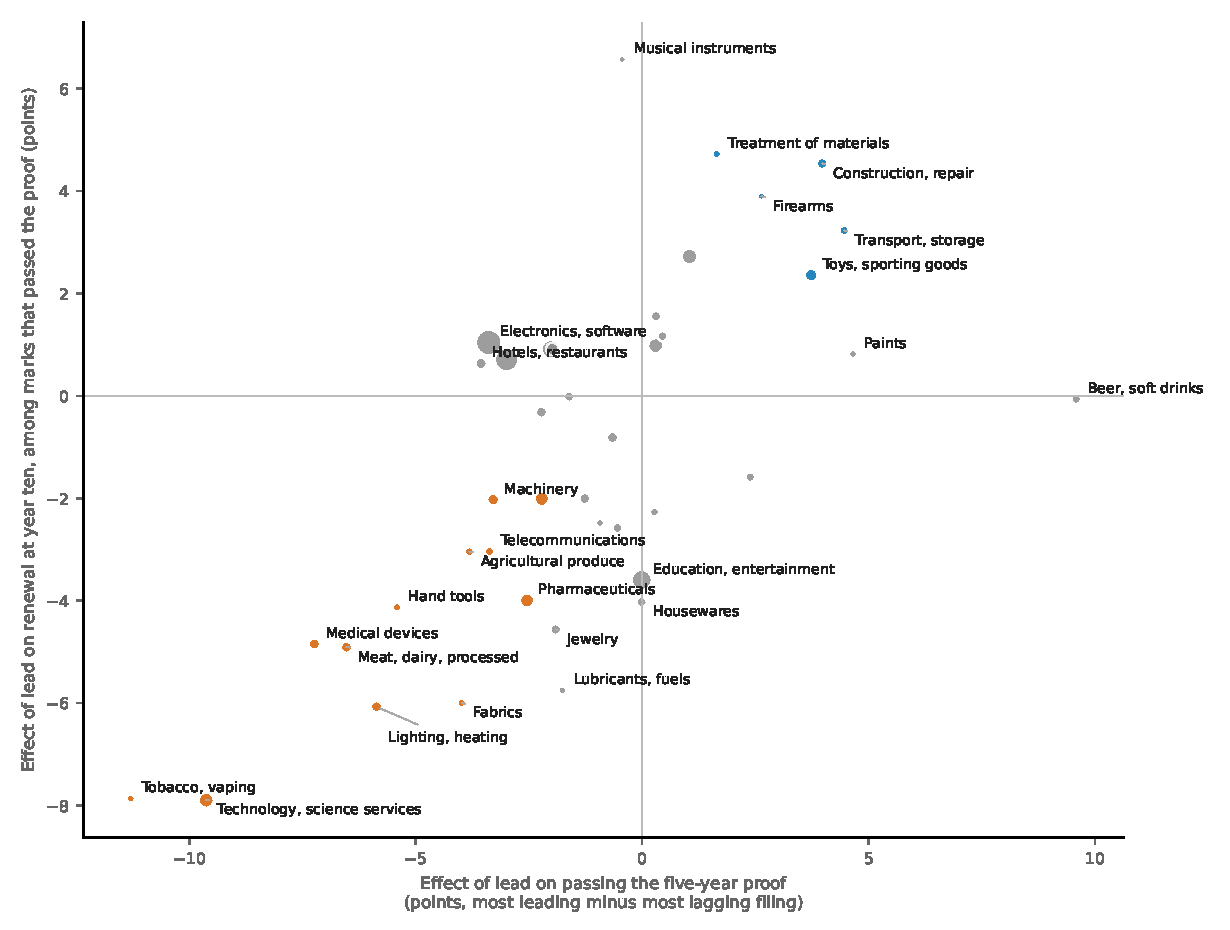
\includegraphics[width=0.85\textwidth]{figures/fig_b_industries.pdf}
\caption{The lead effect by Nice class at the five-year proof and at
renewal among registrations that passed it (top minus bottom of the
class-and-year distribution; class $\times$ registration-year fixed
effects and controls). Orange: leading costs at least 2 points at both
tests; blue: leading pays at least 1.5 points at both. Point size is
proportional to registrations.}
\label{fig:industries}
\end{figure}

\emph{Tobacco's penalty is a change of product.} The class-34 penalty is
confined to registrations of 2013--18 ($-23.4$ points; $+4.1$ and $+0.5$
in 2002--07 and 2008--12), when e-cigarette and vaping language went from
none of the class's registrations to 46\%. Vaping registrations pass the
proof 15.8 points less often than the class's others, and within each
product --- vaping, cigars, cigarettes, hookah --- leading is not
penalized. In class 34 leading language meant vaping, and vaping marks
were abandoned.

\emph{Beer's reward belongs to the craft-beer decade.} In class 32 the
rising product was beer, which went from a third of the class's
registrations in 2002--07 to two-thirds in 2013--18. Beer registrations
pass the proof 7.5 points more often than the class's others, and leading
beer filings 10.1 points more often than lagging ones; at renewal
leading neither helps nor hurts. Across the classes where leading pays,
survival is highest near the 65th percentile of lead and lower at both
ends: the cost there falls on lagging filings, and the most leading tenth
does not gain.

\emph{Where leading pays, unusual language does not.} In the classes
where leading costs least, the most unusual filings pass the proof 2.9
points less often than the most typical; where it costs most,
atypicality has no effect ($+0.7$); in the large middle it is worth 5.8
points. Unusual language pays most in electronics and software ($+16$
points), advertising and business services ($+13$), telecommunications
($+10$) and pharmaceuticals ($+11$), and costs in machinery ($-11$),
legal and personal services ($-7$), chemicals and paints ($-5$).

\section{Discussion: comparing the forces on one scale}\label{sec:discussion}

The literatures on entry order are usually read as a contest between
claims. Measured together on one outcome, the forces they name are all
present, and their sizes differ by an order of magnitude. Retaining
counsel is worth 18.7 points of survival at the five-year proof. Being
unusual for one's industry is worth 4.5 at the proof and 4.3 at
renewal. Being early costs 1.2 for the average registration, and 5 to 11
points for self-filed registrations, platform businesses and a dozen
industries.

\emph{The blue-ocean effect is the larger of the two positions, and it is
contingent on competition.} Language that brings to a class what other
industries describe survives more often, as the practitioner literature
holds \citep{KimMauborgne2004}. The advantage is halved where the
class's filing volume grows by a standard deviation and where the filers
of the same theme concentrate in place, and in fast-growing class-years
only the most unusual filings keep it. Uncontested space pays while it
stays uncontested; growth in entry and concentration of rivals are what
the record shows removing the advantage.

\emph{Protection is specific.} Patents double the advantage of unusual
language and do nothing for the cost of being early, consistent with the
appropriability account, in which protection covers a technology rather
than a position in time \citep{Teece1986}. Counsel
removes the cost of being early and does nothing for the value of being
unusual. Platform businesses keep neither: they pay the most for leading
and keep the least of the atypicality advantage, the reverse of the
network-effects argument for first movers \citep{LiebermanMontgomery1988}.

\emph{Clusters cut both ways.} Concentration of a theme's filers erodes
the value of unusual language, while a theme with an identifiable hub
keeps more of it. The record cannot separate imitation from shared
suppliers, labour or demand; it can say that the two measures move the
advantage in opposite directions and by comparable amounts.

\emph{What the measures cannot say.} Lead and atypicality measure the
position of a filing's language relative to its industry's, not the
novelty of a product, and a mark can lead because others imitated it,
because all responded to the same change, or by coincidence. The
five-year proof records whether goods were still sold under the mark,
not profits. The forced vocabularies were chosen with hindsight. The
co-location measure uses the applicant's address, which for a large firm
may be a headquarters rather than where the product is made. The
estimates are associations within industry and year, with the controls
stated; none identifies a causal effect of choosing unusual or early
language.

\appendix
\section{Every class}\label{app:classes}

Lead and atypicality effects by Nice class (percentage points, top minus
bottom of the class-and-year distribution; standard errors for lead in
parentheses), at the five-year proof (registrations 2002--18) and at
renewal among those that passed (2002--13). A class is placed in a lead
pattern when its effect at a test is at least 2 points (1.5 for
persistent rewards).

{\small\begin{longtable}{r>{\raggedright\arraybackslash}p{3.7cm}rrrrr}
\toprule & & & \multicolumn{2}{c}{Lead} & \multicolumn{2}{c}{Atypicality} \\ \cmidrule(lr){4-5}\cmidrule(l){6-7} Class & & Registrations & Proof & Renewal & Proof & Renewal \\ \midrule \endhead
\addlinespace\multicolumn{7}{l}{\emph{Lead: penalty persists}} \\
34 & Tobacco, vaping & 13,993 & $-$11.3 (2.8) & $-$7.9 (4.5) & +5.1 & $-$3.4 \\
42 & Technology, science services & 127,407 & $-$9.6 (0.6) & $-$7.9 (1.1) & +5.7 & +3.3 \\
10 & Medical devices & 55,537 & $-$7.2 (1.0) & $-$4.8 (1.5) & $-$1.6 & $-$2.1 \\
29 & Meat, dairy, processed & 55,503 & $-$6.5 (1.2) & $-$4.9 (1.8) & $-$0.5 & $-$1.7 \\
11 & Lighting, heating & 55,383 & $-$5.9 (1.1) & $-$6.1 (1.7) & $-$1.0 & +5.2 \\
8 & Hand tools & 19,542 & $-$5.4 (1.6) & $-$4.1 (2.6) & $-$2.4 & $-$4.2 \\
24 & Fabrics & 18,531 & $-$4.0 (1.8) & $-$6.0 (2.9) & +4.2 & +4.5 \\
31 & Agricultural produce & 25,317 & $-$3.8 (1.8) & $-$3.0 (2.7) & +6.8 & +0.8 \\
38 & Telecommunications & 32,421 & $-$3.4 (1.3) & $-$3.0 (2.2) & +10.0 & +11.6 \\
7 & Machinery & 66,181 & $-$3.3 (1.0) & $-$2.0 (1.3) & $-$11.2 & $-$8.8 \\
5 & Pharmaceuticals & 108,181 & $-$2.5 (1.4) & $-$4.0 (1.2) & +10.7 & +7.6 \\
3 & Cosmetics, cleaning & 113,917 & $-$2.2 (0.9) & $-$2.0 (1.4) & +8.1 & +11.1 \\
\addlinespace\multicolumn{7}{l}{\emph{Lead: penalty appears late}} \\
14 & Jewelry & 45,289 & $-$1.9 (1.0) & $-$4.6 (2.0) & +0.7 & $-$4.1 \\
4 & Lubricants, fuels & 11,780 & $-$1.8 (2.6) & $-$5.8 (3.8) & +12.2 & +1.6 \\
21 & Housewares & 40,927 & 0.0 (1.2) & $-$4.0 (1.9) & +3.8 & +5.1 \\
41 & Education, entertainment & 254,579 & 0.0 (0.5) & $-$3.6 (0.8) & 0.0 & $-$0.9 \\
\addlinespace\multicolumn{7}{l}{\emph{Lead: penalty fades}} \\
43 & Hotels, restaurants & 60,493 & $-$3.6 (0.9) & +0.6 (1.6) & $-$2.0 & $-$6.0 \\
9 & Electronics, software & 426,177 & $-$3.4 (0.5) & +1.0 (0.7) & +15.8 & +14.0 \\
35 & Advertising, business & 353,547 & $-$3.0 (0.4) & +0.7 (0.7) & +12.6 & +8.9 \\
1 & Chemicals & 55,166 & $-$2.2 (1.0) & $-$0.3 (1.4) & $-$5.3 & $-$4.2 \\
25 & Clothing & 197,259 & $-$2.0 (0.5) & +0.9 (0.9) & +3.7 & +4.3 \\
\addlinespace\multicolumn{7}{l}{\emph{Lead: benefit persists}} \\
40 & Treatment of materials & 19,797 & +1.7 (1.5) & +4.7 (2.5) & $-$2.3 & $-$2.3 \\
13 & Firearms & 8,387 & +2.6 (2.6) & +3.9 (4.2) & +2.7 & $-$4.6 \\
28 & Toys, sporting goods & 82,356 & +3.7 (1.9) & +2.4 (1.9) & +4.2 & $-$1.7 \\
37 & Construction, repair & 49,178 & +4.0 (1.0) & +4.5 (1.6) & $-$0.9 & $-$3.9 \\
39 & Transport, storage & 30,844 & +4.5 (1.3) & +3.2 (2.1) & +0.4 & +1.3 \\
\addlinespace\multicolumn{7}{l}{\emph{Lead: benefit fades}} \\
45 & Legal, personal services & 34,032 & +2.4 (1.1) & $-$1.6 (2.4) & $-$7.2 & $-$5.0 \\
2 & Paints & 13,215 & +4.7 (2.0) & +0.8 (3.2) & $-$4.8 & $-$3.9 \\
32 & Beer, soft drinks & 37,724 & +9.6 (1.3) & $-$0.1 (2.7) & $-$2.2 & $-$5.8 \\
\addlinespace\multicolumn{7}{l}{\emph{Lead: small}} \\
30 & Coffee, bakery, staples & 79,726 & $-$2.0 (0.9) & +0.9 (1.5) & $-$2.0 & +1.8 \\
20 & Furniture & 43,033 & $-$1.6 (1.1) & 0.0 (1.9) & +2.5 & +5.6 \\
33 & Wine, spirits & 52,838 & $-$1.3 (1.2) & $-$2.0 (2.0) & $-$1.7 & $-$2.0 \\
17 & Rubber, plastics & 14,684 & $-$0.9 (1.7) & $-$2.5 (2.5) & $-$4.9 & $-$0.9 \\
44 & Medical, beauty services & 56,969 & $-$0.7 (0.9) & $-$0.8 (1.7) & $-$3.1 & +0.3 \\
6 & Metal goods & 41,413 & $-$0.5 (1.0) & $-$2.6 (1.5) & $-$2.9 & $-$1.0 \\
15 & Musical instruments & 6,486 & $-$0.4 (2.6) & +6.6 (3.9) & $-$9.1 & +2.3 \\
19 & Building materials & 25,319 & +0.3 (1.5) & $-$2.3 (2.1) & +2.6 & +5.9 \\
16 & Paper, printed matter & 126,216 & +0.3 (0.7) & +1.0 (1.0) & +0.3 & $-$2.6 \\
12 & Vehicles & 43,416 & +0.3 (1.2) & +1.6 (1.7) & $-$0.3 & $-$1.0 \\
18 & Leather goods & 39,283 & +0.4 (1.1) & +1.2 (2.1) & +5.9 & +5.8 \\
36 & Insurance, finance & 141,201 & +1.0 (0.7) & +2.7 (1.1) & $-$0.9 & +0.1 \\
\bottomrule\end{longtable}}


\section{Forced vocabularies}\label{app:vocab}

Each vocabulary is a list of terms matched, case-insensitively, anywhere
in the goods-and-services description.
\begin{description}\small
\item[General-purpose technologies.] Internet: internet, online,
website, web page, world wide web, e-commerce, electronic commerce.
Mobile apps: mobile app(lication), smartphone app, downloadable mobile.
Cloud: cloud computing, cloud-based, software as a service, SaaS,
platform as a service. Social media: social media, social network.
Artificial intelligence: artificial intelligence, machine learning, deep
learning, neural network, natural language processing, computer vision,
chatbot. Blockchain: blockchain, cryptocurrency, bitcoin, non-fungible
token, distributed ledger, virtual currency.
\item[Inventions.] 3D printing and additive manufacturing; drones and
unmanned aerial vehicles; virtual and augmented reality; electric
vehicles and EV charging; gene therapy, gene editing, CRISPR;
nanotechnology, nanoparticles, nanomaterials.
\item[Emergent consumer categories.] Electronic cigarettes and vaping;
energy drinks; kombucha; cold brew; plant-based, almond, oat and
non-dairy milk; hard and alcoholic seltzer; cannabidiol, CBD,
hemp-derived.
\item[Kinds of business.] Site-based: restaurant, hotel, motel, retail
store, store services, clinic, salon, spa, fitness center or club, gym,
bar services, cafe, car wash, day or child care, dental, veterinary,
coffee shop, bakery services. Contract or subscription: subscription,
membership, account(s), insurance, banking, telecommunication, leasing,
financing. Platform: platform(s), marketplace, social network, online
community, peer-to-peer, connecting buyers, users or people.
\end{description}

\begin{thebibliography}{99}

\bibitem[Duranton \& Overman(2005)]{DurantonOverman2005}
Duranton, G., \& Overman, H.~G. (2005). Testing for localization using
micro-geographic data. \emph{Review of Economic Studies}, 72(4),
1077--1106.

\bibitem[Golder \& Tellis(1993)]{GolderTellis1993}
Golder, P.~N., \& Tellis, G.~J. (1993). Pioneer advantage: Marketing logic or
marketing legend? \emph{Journal of Marketing Research}, 30(2), 158--170.

\bibitem[Kim \& Mauborgne(2004)]{KimMauborgne2004}
Kim, W.~C., \& Mauborgne, R. (2004). Blue ocean strategy. \emph{Harvard
Business Review}, 82(10), 76--84.

\bibitem[Klepper(1997)]{Klepper1997}
Klepper, S. (1997). Industry life cycles. \emph{Industrial and Corporate
Change}, 6(1), 145--182.

\bibitem[Klepper \& Miller(1995)]{KlepperMiller1995}
Klepper, S., \& Miller, J.~H. (1995). Entry, exit, and shakeouts in the
United States in new manufactured products. \emph{International Journal
of Industrial Organization}, 13(4), 567--591.

\bibitem[Lieberman \& Montgomery(1988)]{LiebermanMontgomery1988}
Lieberman, M.~B., \& Montgomery, D.~B. (1988). First-mover advantages.
\emph{Strategic Management Journal}, 9(S1), 41--58.

\bibitem[Lieberman \& Montgomery(1998)]{LiebermanMontgomery1998}
Lieberman, M.~B., \& Montgomery, D.~B. (1998). First-mover (dis)advantages:
Retrospective and link with the resource-based view. \emph{Strategic
Management Journal}, 19(12), 1111--1125.

\bibitem[Robinson \& Fornell(1985)]{RobinsonFornell1985}
Robinson, W.~T., \& Fornell, C. (1985). Sources of market pioneer advantages
in consumer goods industries. \emph{Journal of Marketing Research}, 22(3),
305--317.

\bibitem[Semadeni \& Anderson(2010)]{SemadeniAnderson2010}
Semadeni, M., \& Anderson, B.~S. (2010). The follower's dilemma:
Innovation and imitation in the professional services industry.
\emph{Academy of Management Journal}, 53(5), 1175--1193.

\bibitem[Silver(2026)]{SilverCorpus2026}
Silver, E. (2026). An event-dated corpus of US trademark prosecution and
a two-sided measure of vocabulary position. SSRN Working Paper 7520758.
\url{https://ssrn.com/abstract=7520758}.

\bibitem[Su\'arez \& Lanzolla(2007)]{SuarezLanzolla2007}
Su\'arez, F.~F., \& Lanzolla, G. (2007). The role of environmental
dynamics in building a first mover advantage theory. \emph{Academy of
Management Review}, 32(2), 377--392.

\bibitem[Teece(1986)]{Teece1986}
Teece, D.~J. (1986). Profiting from technological innovation:
Implications for integration, collaboration, licensing and public
policy. \emph{Research Policy}, 15(6), 285--305.

\end{thebibliography}

\end{document}
